En el siguiente capítulo se revisarán algunos conocimientos previos que serán útiles para poder tener un mejor entendimiento tanto del problema de investigación como de la solución que se planteará. Entre estos conocimientos previos, se explicarán a detalle algunos de los modelos del estado del arte en temas de clasificación de imágenes utilizando ML, el procedimiento de \textit{transfer learning}(TL) y \textit{continuous learning} CL, las restricciones de un sistema a tiempo real, el pre-procesamiento de las entradas y el \textit{dataset} que se planea utilizar para este trabajo.\\

\section{Modelos de \textit{Machine Learning} para clasificación}
ML ha evolucionado a lo largo del tiempo, de tal manera que ahora los diferentes modelos pueden realizar trabajos mas complejos hasta el punto de sobrepasar en eficiencia y precisión a los humanos en algunas tareas. Dentro de estas tareas, las de clasificación son una de las áreas mas investigadas y la cual también presenta varias aplicaciones en el mundo real. Dentro de esta tarea, el \textit{Multi Layer Perceptron} (MLP) y las \textit{Convolutional Neural Networks} (CNN) son las dos arquitecturas dentro del estado del arte para el análisis de imágenes.

\subsection{\textit{Multi Layer Perceptron} (MLP)}
Tal como lo dice su nombre, esta arquitectura consiste de múltiples capas de neuronas artificiales, las cuales reciben la data a ser procesada y es pasada por una función de activación, para que se conviertan en la entrada de la siguiente capa. Este proceso imita el trabajo de las neuronas humanas como se puede ver en la figura \ref{neurona}. \\

\begin{figure}[h!]
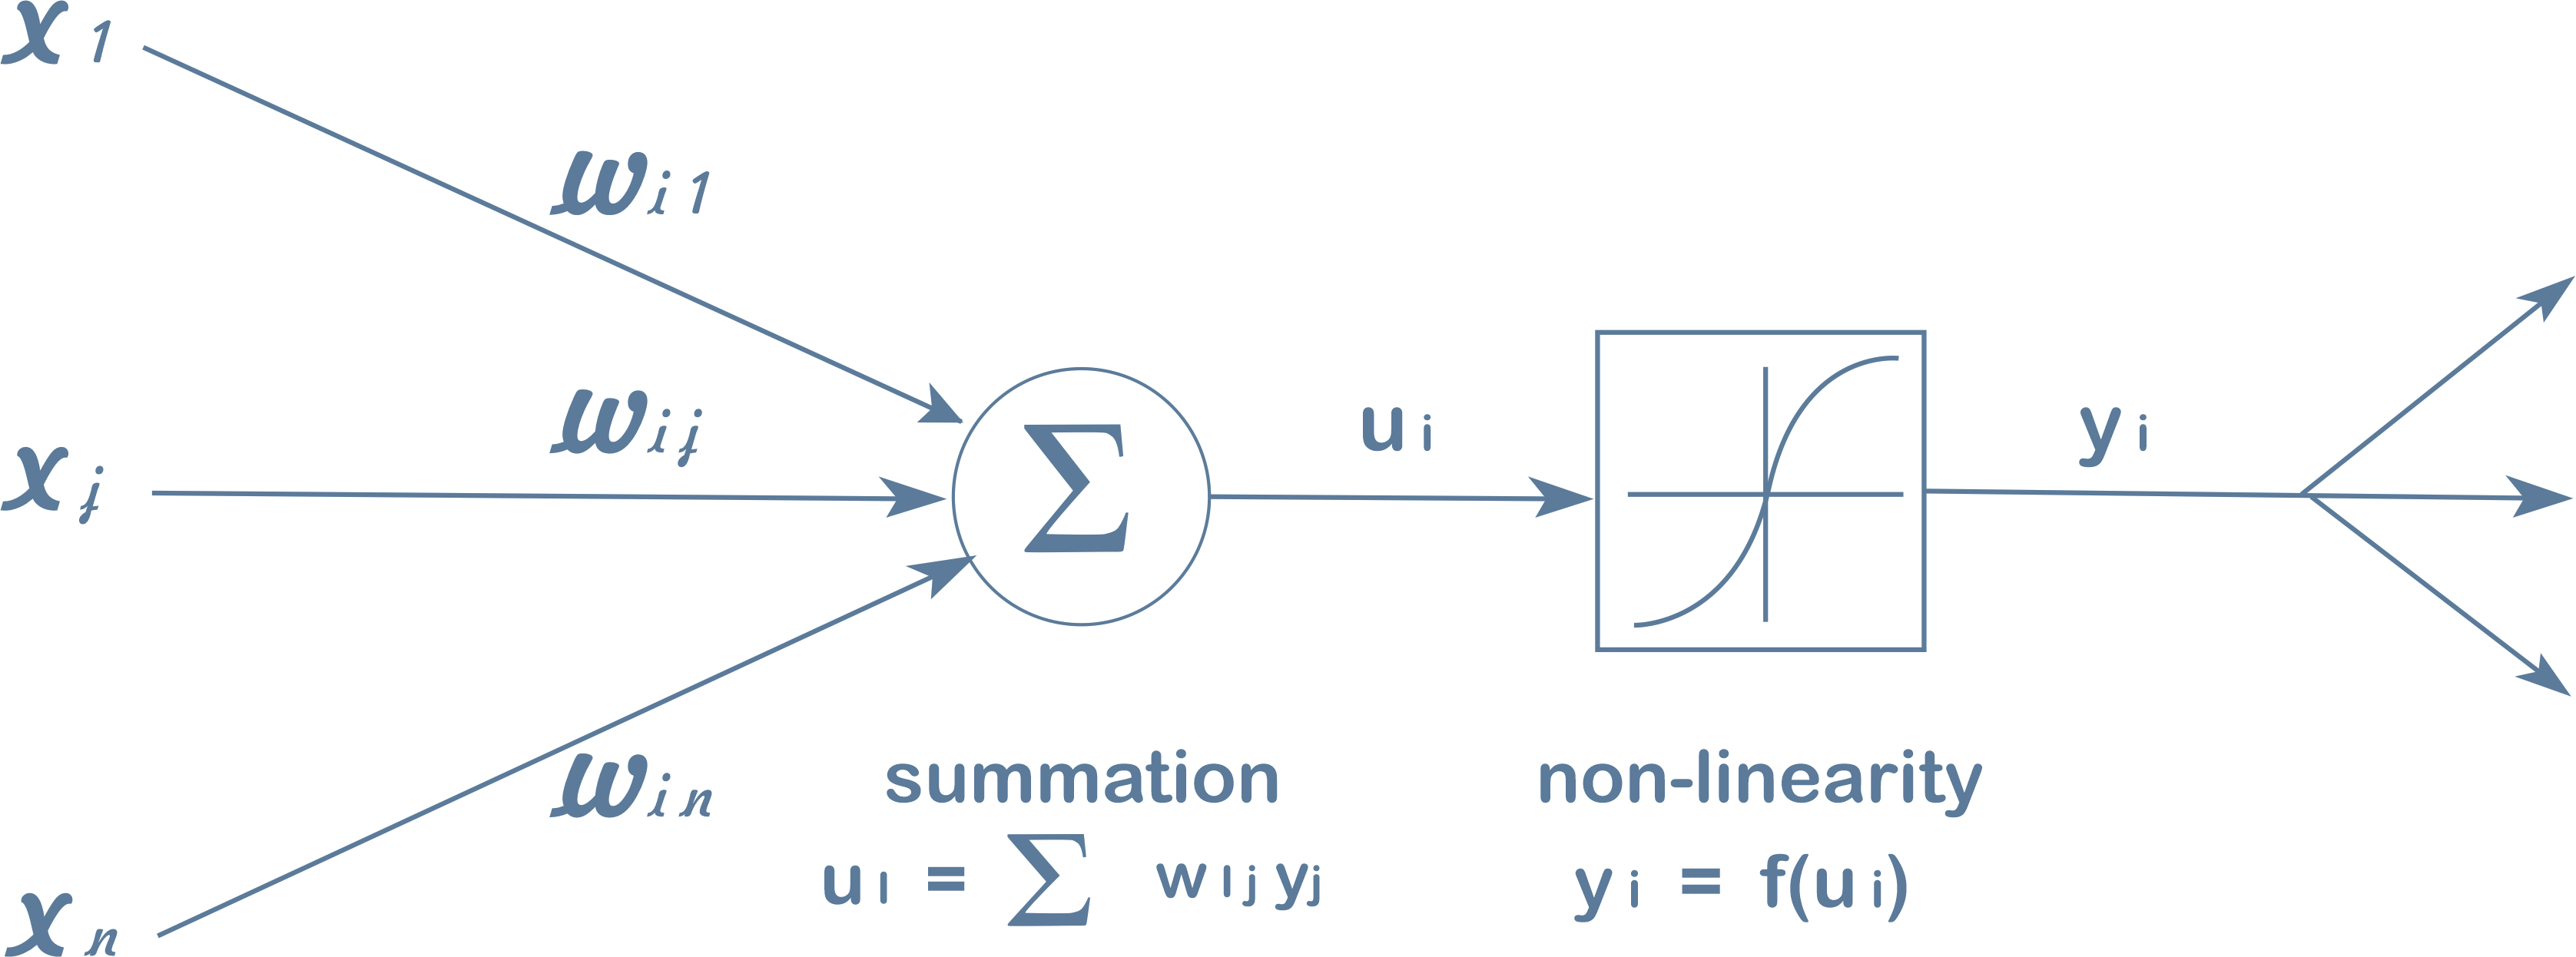
\includegraphics[width=0.8\textwidth]{images/comparacion_neuronas.jpg}
\centering
\caption{Comparacion entre una neurona real y una artificial\protect\cite{neuronas}.}
\label{neurona}
\end{figure}

Una MLP consta de varias capas ``densas'' de neuronas conectadas entre ellas. Una vez realizado el procesamiento de las entradas por toda la red neuronal, comienza el proceso de modificación de los pesos \textit{w} de cada una de las capas. Este proceso se llama ``retro propagación'' o \textit{back propagation} y como lo dice su nombre, se basa en propagar las derivadas de cada una de las funciones de las neuronas desde la última capa hasta la primera.\\\\
Este modelo espera como entrada un vector de características o de información, en ese sentido, no es especialmente bueno para poder analizar información como imágenes ya que realizar este proceso sería demasiado complejo computacionalmente hablando al tener una imagen de alta calidad, también por el hecho de que la extracción de características ya esta omitiendo información y, por último, que la información de una imagen suele cumplir el principio de localidad (la información relevante suele estar reunida en espacios cercanos) y vectorizarla estaría omitiendo características importantes para su análisis.

\subsection{\textit{Convolutional Neural Networks} (CNN)}

Las CNN's son modelos basados en una arquitectura  especialmente diseñadas para el análisis de imágenes y en especial, su clasificación. Ellas realizan la labor de extracción de características que no realiza el MLP a través de convoluciones. Esto evita la perdida de información y mejoran su eficiencia y precisión sobre todo. \\

Las convoluciones se basan en un procedimiento que permite extraer características al aplicar una matriz cuadrada de transformación (generalmente bastante pequeña) a lo largo de la imagen original, la cual luego devuelve otra imagen modificada. Estas matrices de transformación son llamadas kernels. En la figura \ref{convolucion} se ilustra una iteración de la convolución .

\begin{figure}[h!]
\includegraphics[width=0.7\textwidth]{images/convolución.png}
\centering
\caption{Proceso de convolución simplificado\protect\cite{convoluciones}.}
\label{convolucion}
\end{figure}

Por otra parte, existen otras capas importantes, los \textit{poolings}, como se ilustra en la imagen \ref{pooling}. Estas capas consisten de la aplicación de una lógica a un cuadrante de la matriz resultante de las convoluciones. Esta lógica varía dependiendo de las necesidades del usuario. En la imagen mencionada anteriormente se puede ver la comparación entre el \textit{Max Pooling} y el \textit{Average Pooling}, las cuales tal como dicen sus nombres, obtienen el máximo y el promedio de los cuadrantes seleccionados para generar un nuevo resultado de menor dimensión. 

\begin{figure}[h!]
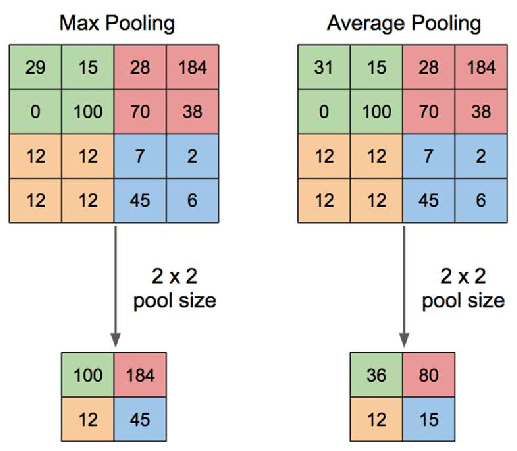
\includegraphics[width=0.6\textwidth]{images/pooling.png}
\centering
\caption{Proceso de convolución simplificado\protect\cite{pooling}.}
\label{pooling}
\end{figure}

Las CNN's se conforman por la unión de capas convolucionales y \textit{pooling} repetidas veces, terminando en una MLP, la cual realiza el trabajo final del procesamiento de las características extraídas. En la imagen \ref{CNN} se puede ver la estructura de una CNN. Como se mencionó anteriormente, el proceso de la extracción de características se realiza dentro de la misma red neuronal, evitando perdida de información a comparación de la MLP, dejándole a esta unicamente el trabajo de la clasificación.

\begin{figure}[h!]
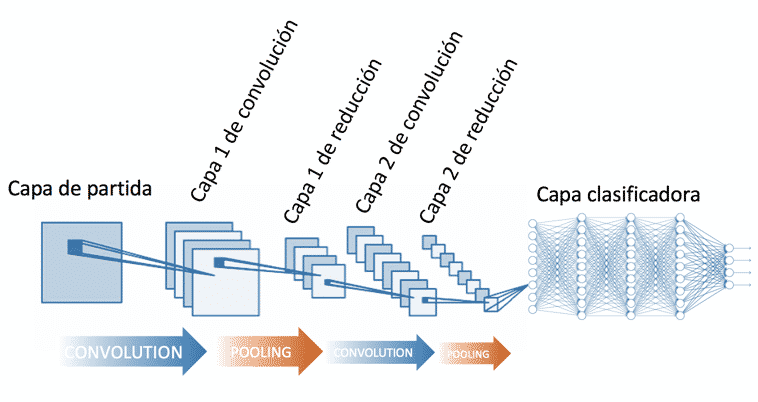
\includegraphics[width=1\textwidth]{images/CNN.png}
\centering
\caption {Arquitectura general de una CNN\protect\cite{CNN-Arquitectura}. }
\label{CNN}
\end{figure}



\section{Arquitecturas del estado del arte}

\subsection{VGG-19}
Esta es una red neuronal convolucional que tiene 19 capas de profundidad. Fue construido y entrenado por Karen Simonyan y Andrew Zisserman\cite{Simonyan2015} en la Universidad de Oxford en 2014, y posteriormente publicado en 2015. Su versión detallada se ilustra en la imagen \ref{VGG19}. Este modelo fue utilizado para intentar clasificar las imagenes del \textit{dataset} ImageNet, llegando a clasificar hasta 1000 objetos diferentes. Como mencionamos anteriormente, cada uno de los modelos necesita una entrada especifica. En este modelo se espera una imagen de 224x224 píxeles para su procesamiento. Debido a su profundidad, este modelo es bastante pesado, llegando a consumir 550 MB de memoria con alrededor de 143 millones de características. Cabe resaltar que el 70\% de todas estas características son debido al paso entre la última capa convolucional y la primera de clasificación. Con todas estas características, logró obtener un resultado de 90\% de precisión con ImageNet.

\begin{figure}[h!]
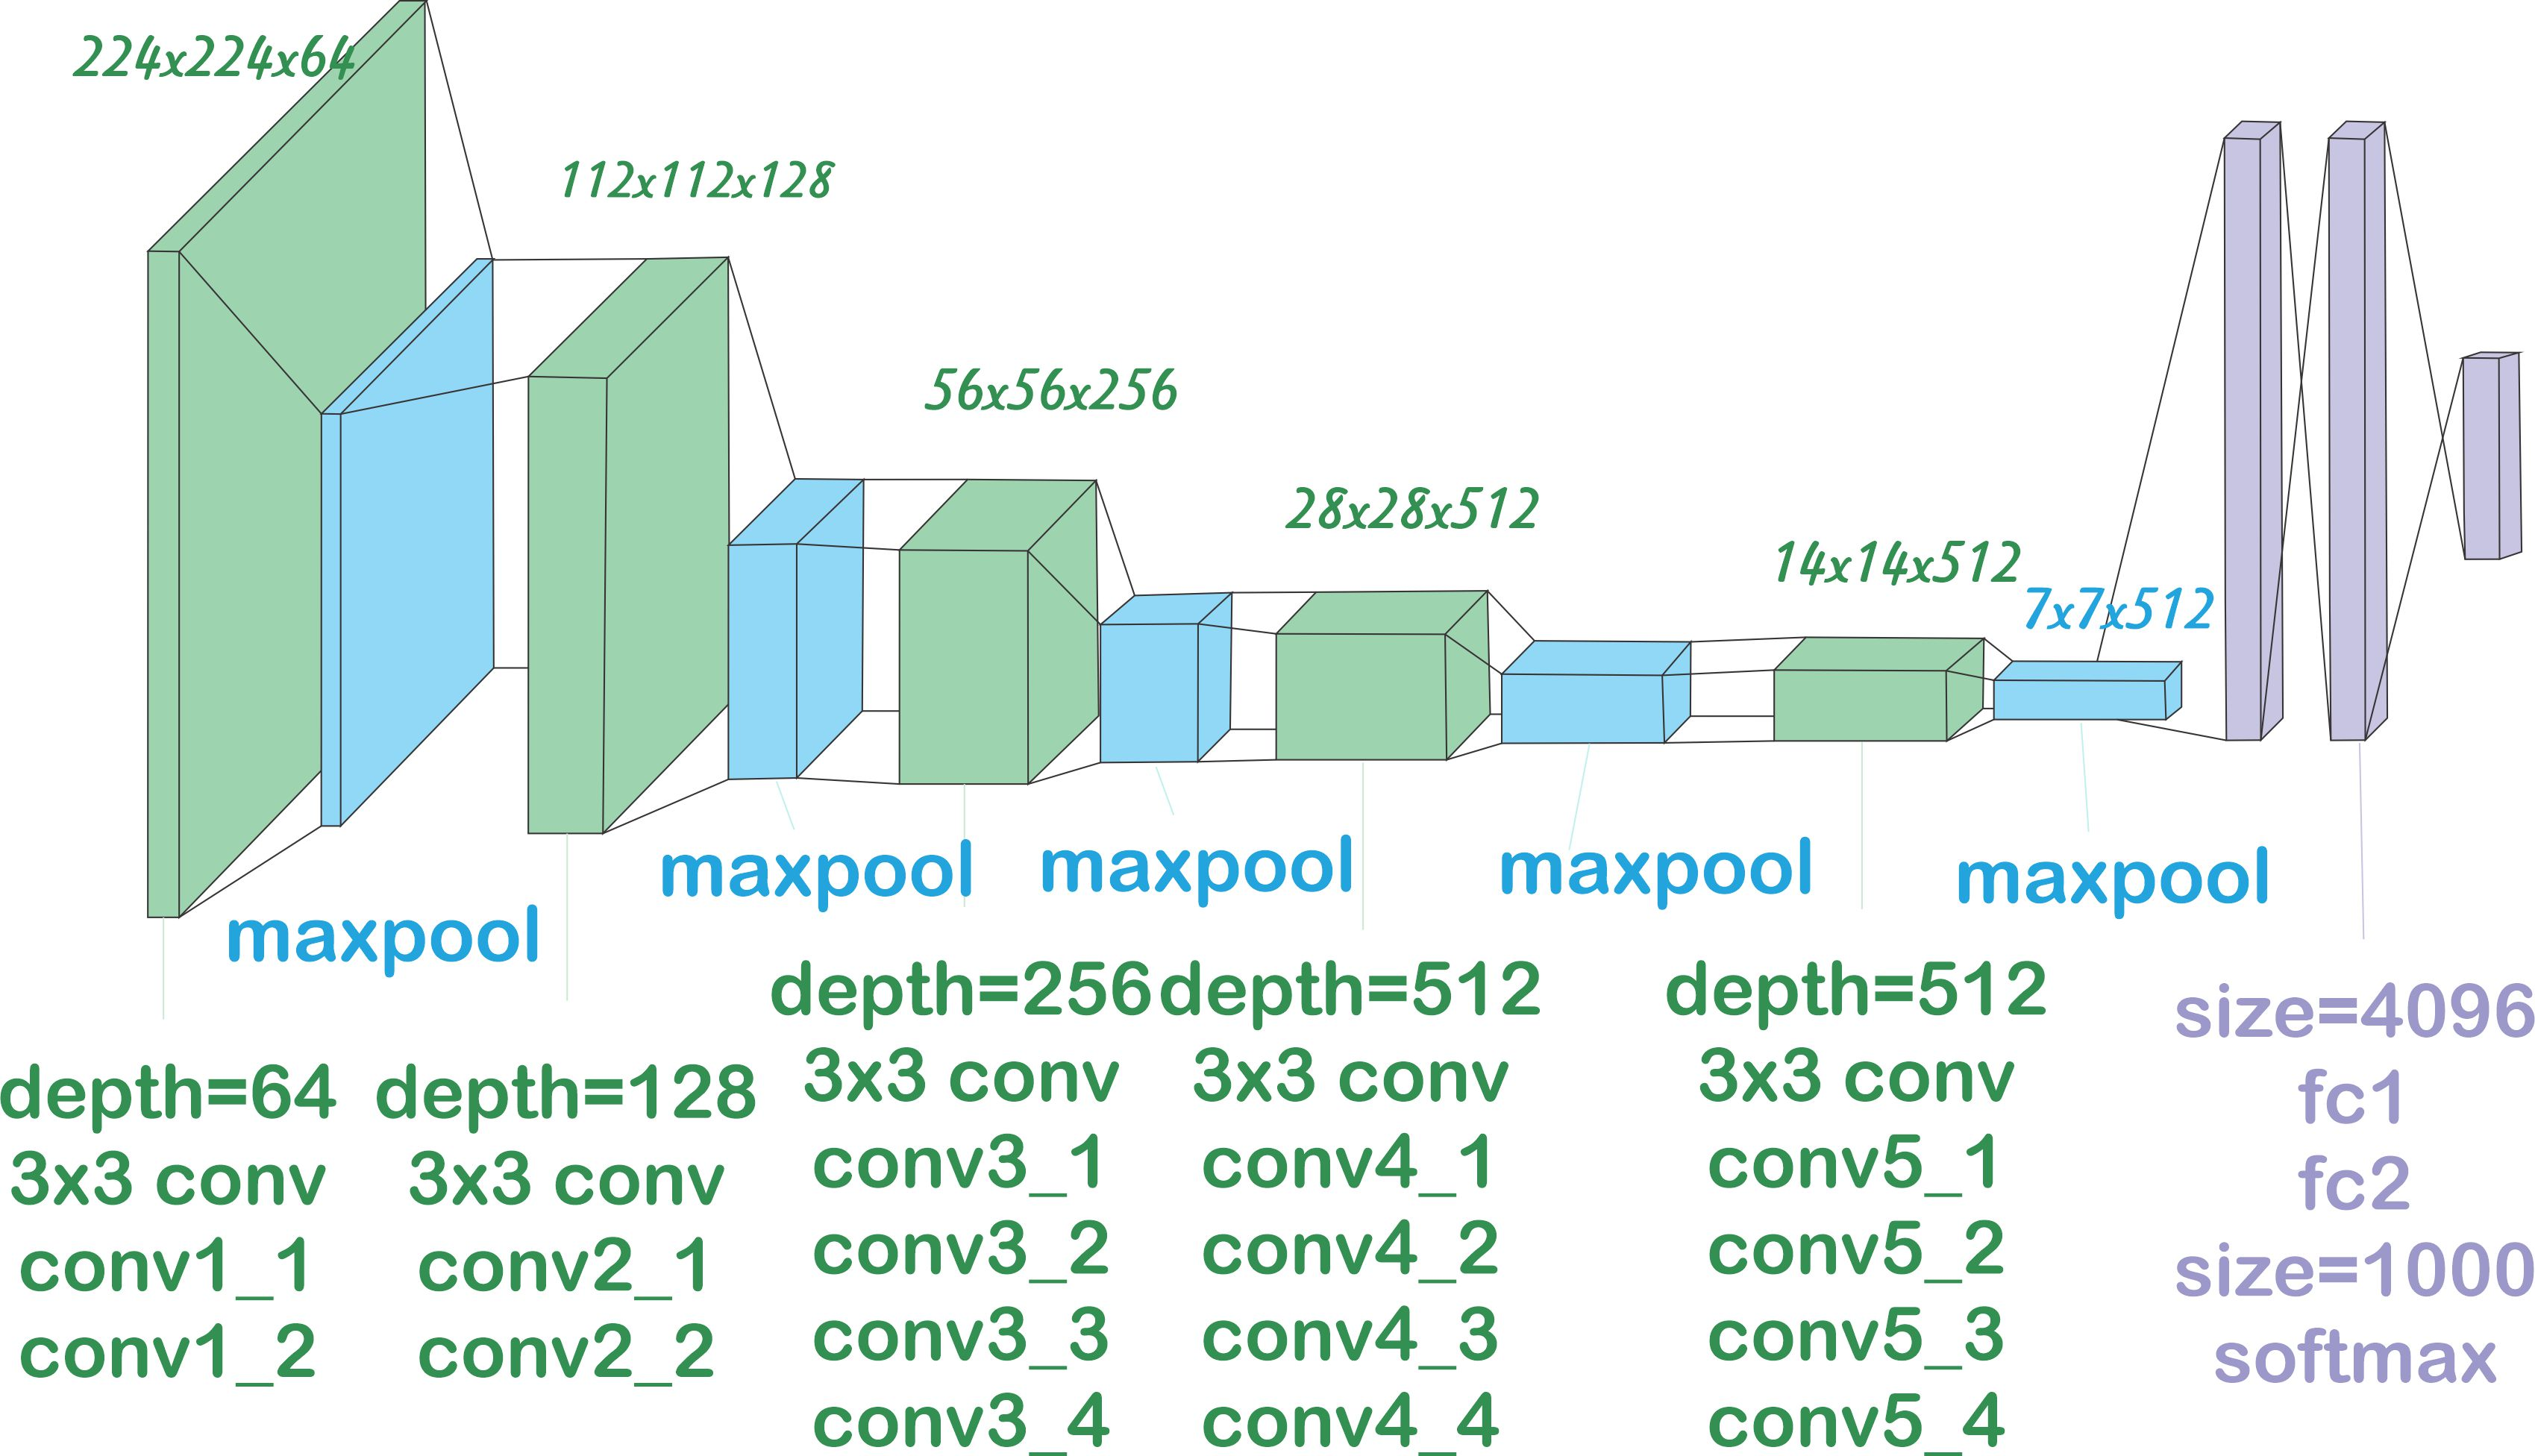
\includegraphics[width=1\textwidth]{images/VGG19.jpeg}
\centering
\caption{Versión simplificada de VGG19 \protect\cite{modelos}. }
\label{VGG19}
\end{figure}

\subsection{InceptionV3}
Si bien la anterior red lograba obtener una precisión muy elevada, esta consumía demasiados recursos. Es por ello que Google desarrolló InceptionV3, una red que prometió obtener los mismos resultados pero con menor costo. Presentado en "\textit{Going deeper with convolutions}" \cite{Szegedy2014}, este modelo alcanza una precisión del 93.7\% con el mismo \textit{dataset}. \\\\
Si bien esta red contiene 50 capas de profundidad (las cuales superan a las de la VGG19), el numero de características a entrenar era menor (23.8 millones). Esto es debido a que esta red proponía que realizar convoluciones unidimensionales como se ve en la figura \ref{InceptionLayer} en serie equivalían a realizar una bidimencional, pero con menores costos. En ese sentido disminuyeron la complejidad que se tenía en los modelos de CNN convencionales, haciéndolo mas ligero y aumentando la capacidad de aprendizaje del modelo. En total, este modelo llega a pesar 92 MB, lo cual es alrededor de 6 veces menor que el anterior. Su entrada requiere de imágenes de 299x299 píxeles y su arquitectura se ve reflejada en la figura \ref{Inceptionv3}

\begin{figure}[h!]
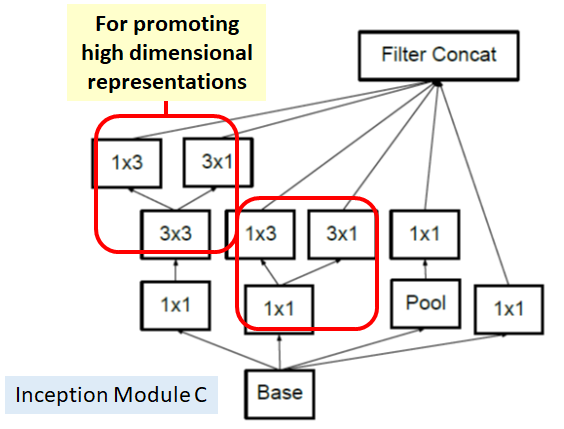
\includegraphics[width=0.8\textwidth]{images/InceptionLayer.png}
\centering
\caption{Reducción de la dimensionalidad del InceptionV3. \protect\cite{modelos} }
\label{InceptionLayer}
\end{figure}

\begin{figure}[h!]
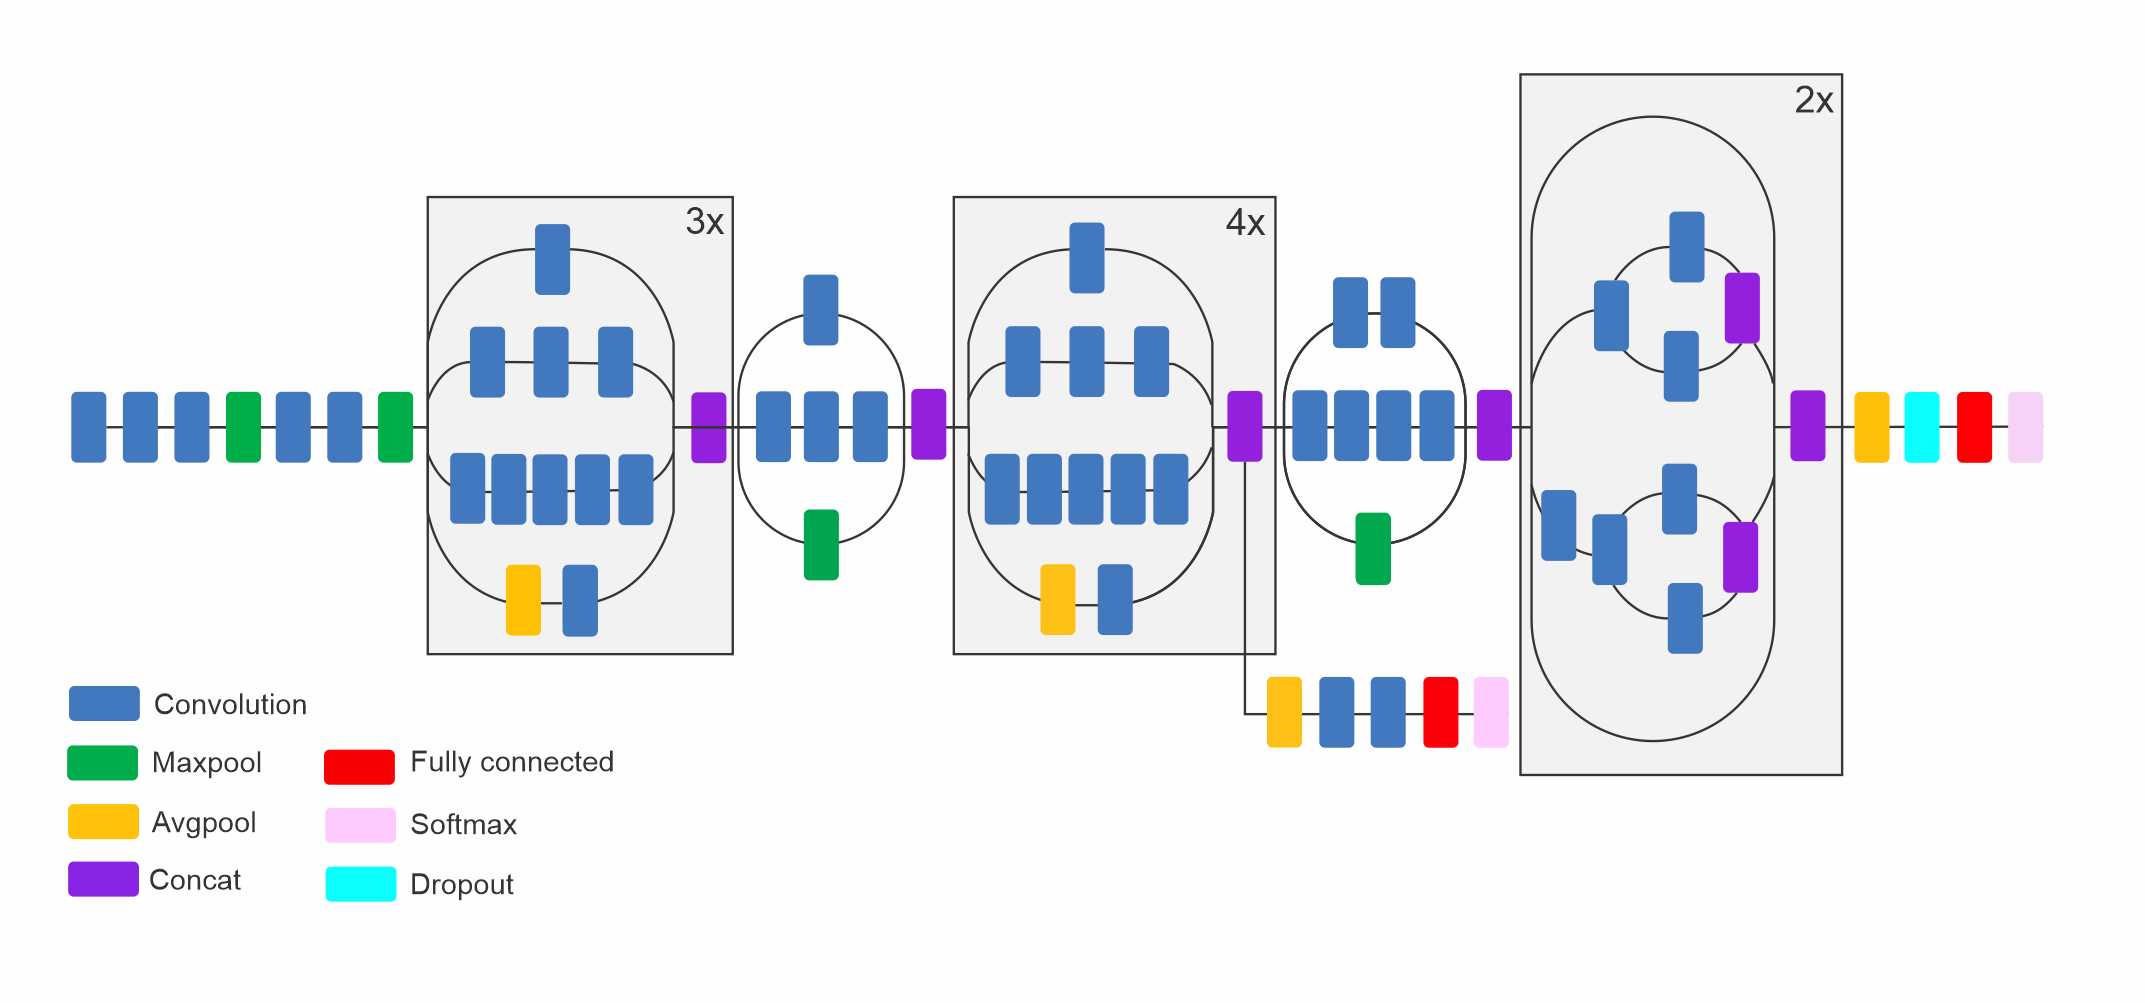
\includegraphics[width=1\textwidth]{images/InceptionV3.png}
\centering
\caption{Versión simplificada de InceptionV3. \protect\cite{modelos} }
\label{Inceptionv3}
\end{figure}

\subsection{ResNet50}
Creada por Microsoft en 2015, cuenta también con 50 capas profundas. Este modelo emplea lo que se le llama `aprendizaje residual' \cite{He2015}, la cual consiste en guardar una copia de lo aprendido actualmente, y sumarlo al resultado después de aplicar una cantidad de convoluciones (en este caso cada tres). La imagen \ref{ResNet} ilustra esta modificación dentro del modelo además de su arquitectura general. Este modelo también fue probado con el mismo \textit{dataset} obteniendo un 92.1\% de precisión y gracias al aprendizaje residual se evito aumentar la dimensionalidad del modelo. Esta red contiene 25.6 millones de características aproximadamente y llega a ocupar 98MB de memoria. 

\begin{figure}[h!]
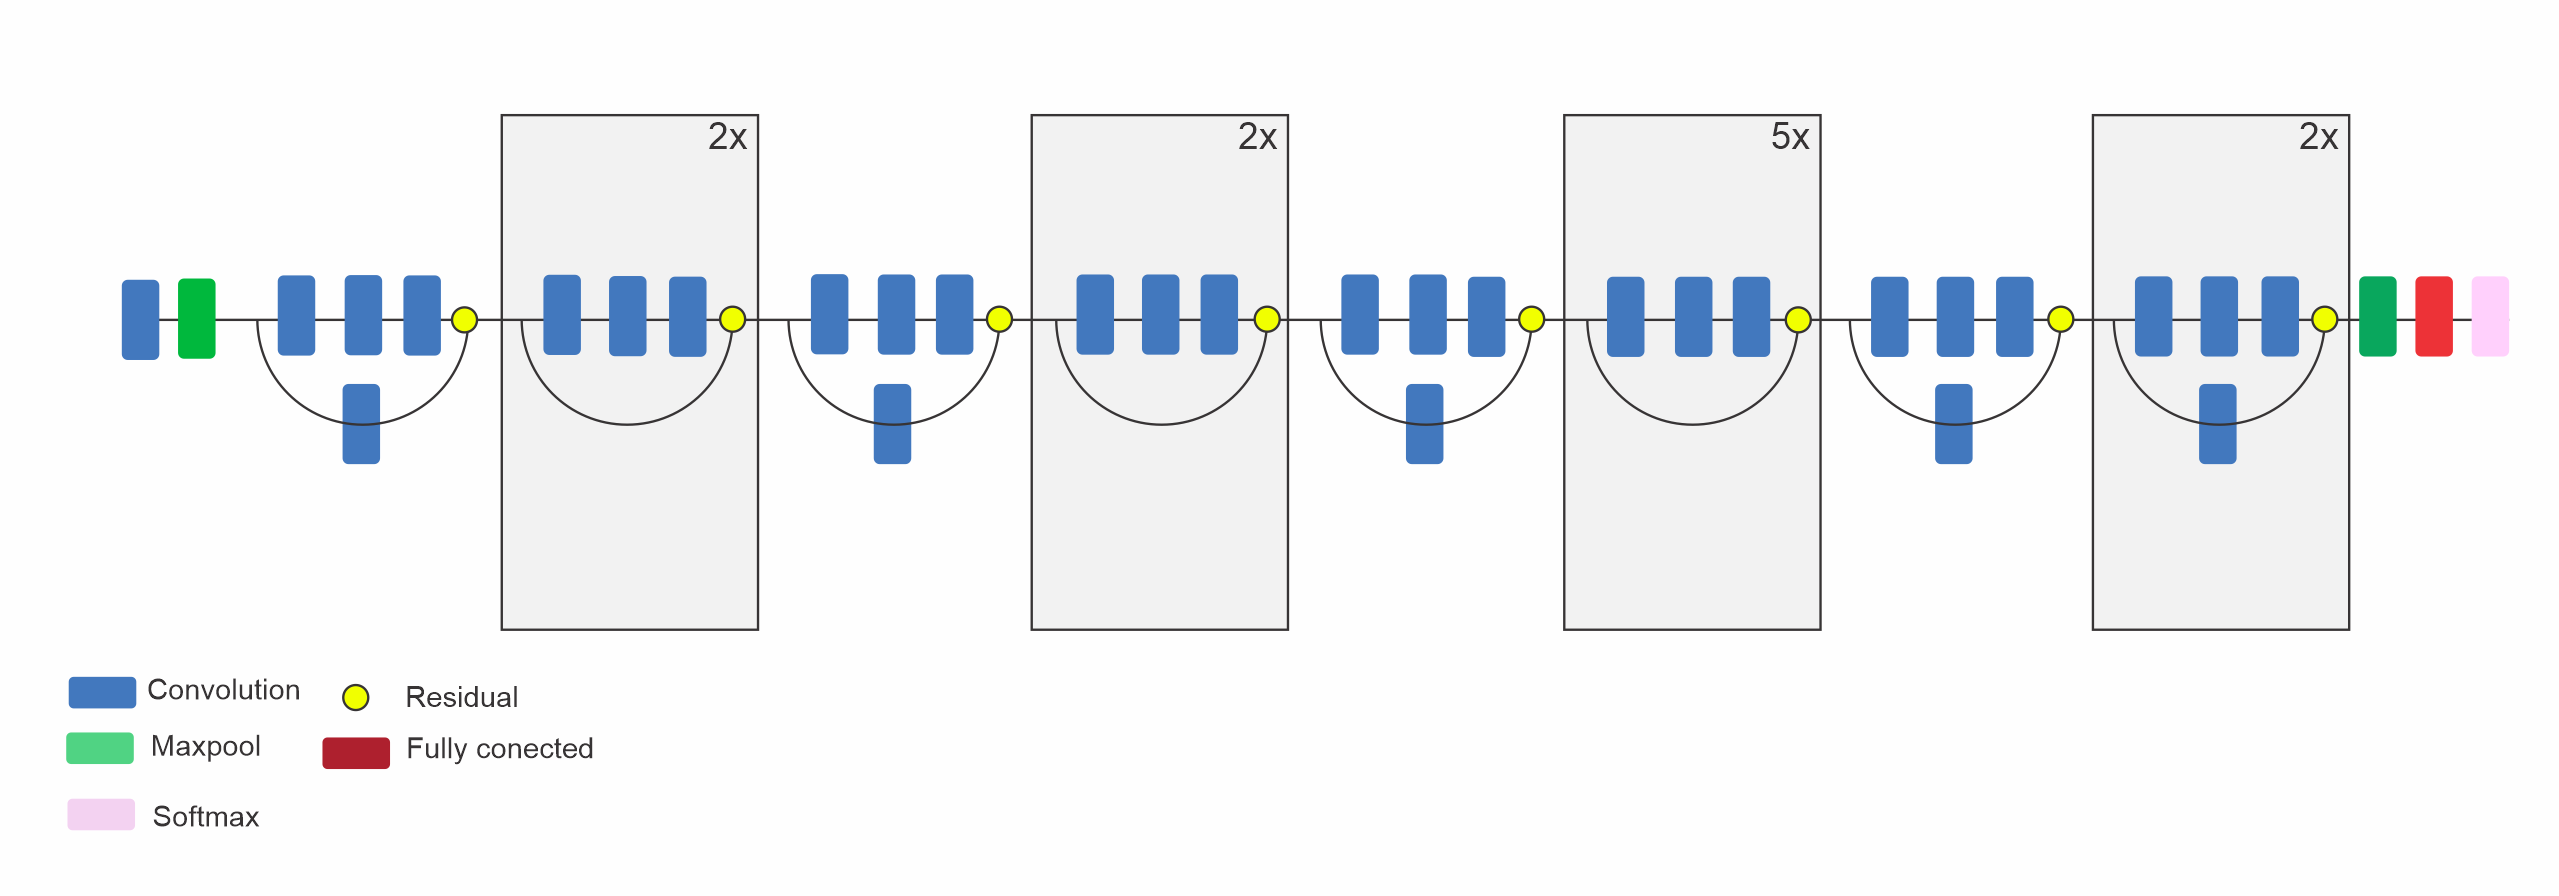
\includegraphics[width=1\textwidth]{images/ResNet.png}
\centering
\caption{Versión simplificada de ResNet50. \protect\cite{modelos} }
\label{ResNet}
\end{figure}


\subsection{EfficientNet}

Creada por Google en 2019 y publicada en " \textit{EfficientNet: Rethinking Model Scaling for Convolutional Neural Networks}" \cite{Tan2020} en 2020 consta de ocho implementaciones diferentes (B0 a B7). La implementación mas liviana (B0) consiste de 5.5 millones de características aproximadamente siendo probada en el mismo \textit{dataset} con una precisión de 93\%. Las demás implementaciones continúan aumentando el numero de características y a su vez la precisión que obtienen. Haciendo una comparación con los anteriores modelos, EfficientNetB4, el cual consta de 19.5 millones de características, genera una precisión de 96.4\%, superándolos. La manera en la que este modelo optimiza su propio aprendizaje es a través de un algoritmo de aproximación que permite generar parámetros para la creación de cada uno de los ocho modelos. Este algoritmo toma en cuenta 3 factores:

\begin{itemize}
    \item Profundidad de las capas
    \item Ancho de las capas (multicapa)
    \item Resolución de las imágenes
\end{itemize}
En la figura \ref{EfficientNetB0} se puede ver la estructura de la EfficientNetB0. 


\begin{figure}[h!]
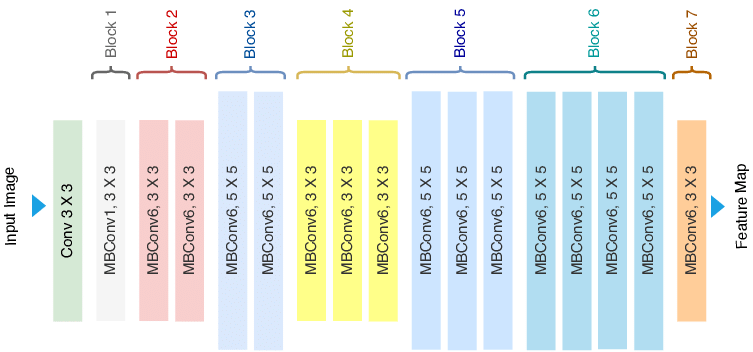
\includegraphics[width=1\textwidth]{images/EfficientNetB0.png}
\centering
\caption{Versión simplificada de EfficientNetB0. \protect\cite{EfficientNetB0} }
\label{EfficientNetB0}
\end{figure}

\subsection{YOLO}
YOLO (\textit{you only look once}) se presenta como una arquitectura que permite ``predecir simultáneamente múltiples cuadros delimitadores (\textit{bounding boxes}) y probabilidades de su clase para ellos'' \cite{Redmon2015}. Este modelo se basa en una CNN convencional, la cual a comparación de implementaciones previas(R-CNN y FR-CNN) realiza la predicción de los \textit{bounding boxes} de manera interna, permitiendo una menor latencia, creando un modelo factible para su uso en tiempo real.\\\\
Este calculo se realiza en base a la generación de grillas (\textit{grids}) o secciones de la imagen, dentro de las cuales se inicializan un número de \textit{bounding boxes} predeterminados, ambos siendo hiperparámetros de la arquitectura. Esta es replicable utilizando cualquier arquitectura de CNN como base, como por ejemplo alguna de las anteriormente mencionadas, solamente ajustando la salida y hiperparámetros correspondientes. Versiones más modernas obtienen una mejor capacidad de detección, módulos de atención, entre otras variaciones que lo hacen cada vez más robustos. En la imagen \ref{YOLO} se puede ver ejemplificada la arquitectura del modelo yolov5.

\begin{figure}[h!]
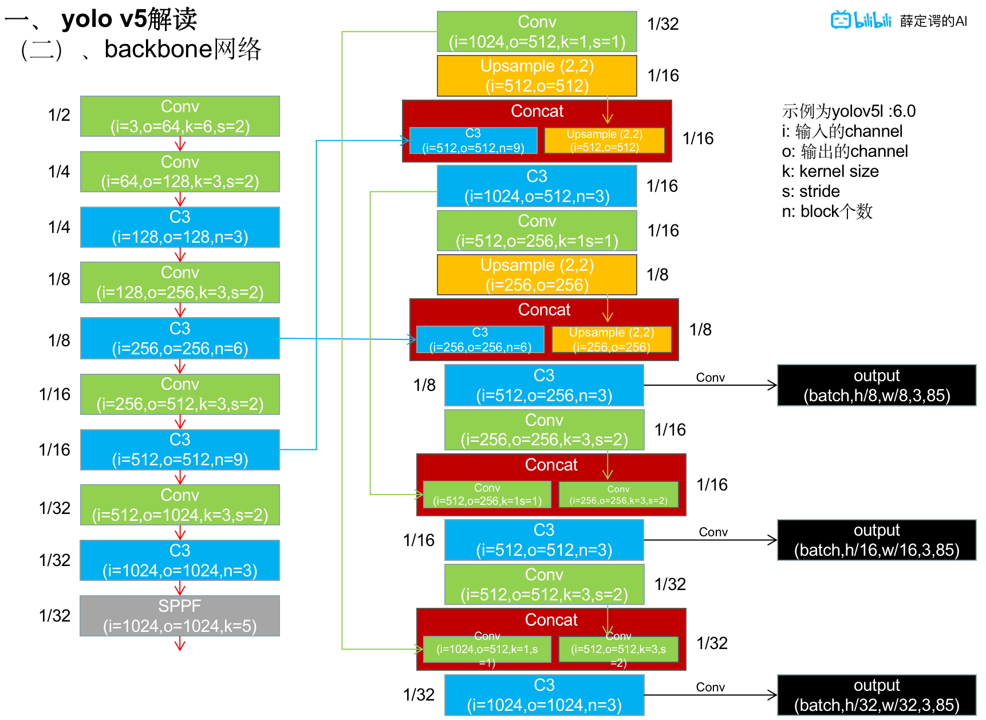
\includegraphics[width=1\textwidth]{images/yolov5.png}
\centering
\caption{Representación de la arquitectura YOLOV5 \protect\cite{yolov5}}
\label{YOLO}
\end{figure}

\subsection{UniDet}

UniDet (\textit{Unified Detector}) fue presentado en el año 2022 e intenta resolver el problema de la unificación de \textit{datasets} para la creación de un modelo robusto que logre también predecir en \textit{datasets} externos a los de entrenamiento, generando una precisión comparable al estado del arte. Esta arquitectura consta de un \textit{backbone} (extractor de características), que pasa después a tres diferentes \textit{heads} (quien realiza la detección y clasifica el \textit{bounding box} por cada dataset para luego finalmente generar una respuesta unificada. Esta arquitectura se puede resumir en la imagen \ref{fig:unidet}

\begin{figure}[h!]
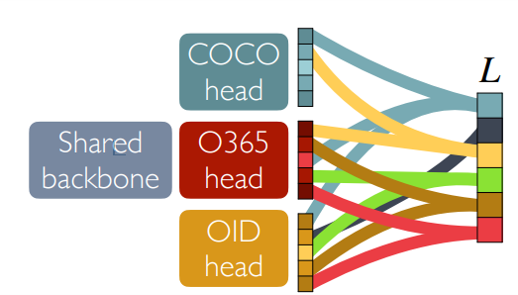
\includegraphics[width=1\textwidth]{images/imagenUnidet.png}
\centering
\caption{Representación de la arquitectura UniDet \protect\cite{unidet}.}
\label{fig:unidet}
\end{figure}

El \textit{backbone} esta basado en una arquitectura Cascade RCNN, el cuál consiste de usos recursivos de capas convolucionales, \textit{heads} y generación de predicciones para manejar imágenes borrosas utilizando una técnica de \textit{resampling} a través de la recursividad mencionada. La arquitectura de este modelo está resumida en la imagen \ref{fig:cascade}

\begin{figure}[h!]
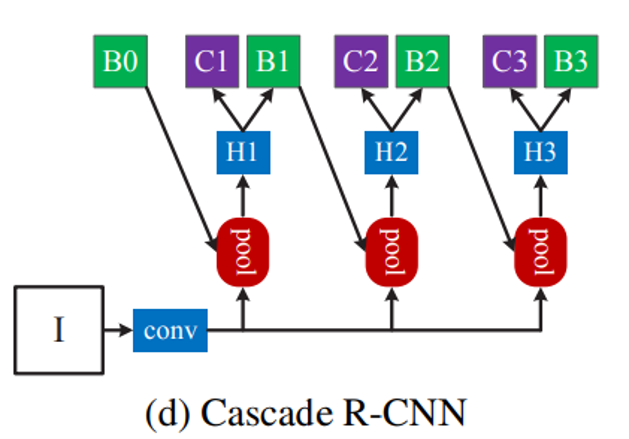
\includegraphics[width=0.6\textwidth]{images/cascadercnn.png}
\centering
\caption{Representación de la arquitectura Cascade RCNN \protect\cite{cascadercnn}.}
\label{fig:cascade}
\end{figure}

Esta arquitectura representa el estado del arte en el tema de detección y clasificación en la mayoría de los \textit{datasets} más comunes tales como COCO, Objects365, Open Images, VOC, VIPER, entre otros.  

\section{\textit{Transfer Learning}}
Según Muhamad Yani\cite{Yani2019}, se le llama \textit{Transfer Learning(TL)} al ``proceso de la transferencia del conocimiento de un entrenamiento previo para ser usado en una nueva para la reducción de tiempo en el proceso de aprendizaje''. En la figura \ref{transfer-learning} se puede evidenciar este proceso.\\ 

\begin{figure}[h!]
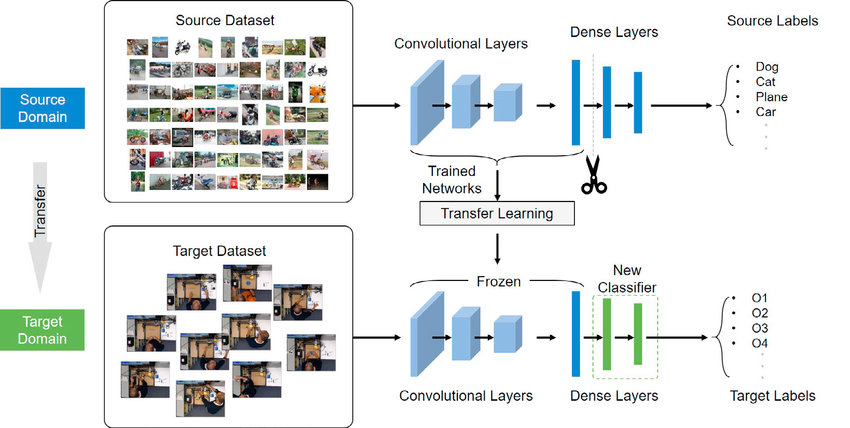
\includegraphics[width=1\textwidth]{images/transfer-learning.png}
\centering
\caption{Comparación entre el aprendizaje común y transfer learning. \protect\cite{transfer-learning}}
\label{transfer-learning}
\end{figure}

Transfer Learning difiere al proceso convencional de entrenamiento de una red ya que no es necesario entrenarlo con un \textit{dataset} grande. En contraste con el proceso convencional, se congelan las capas iniciales del modelo (en nuestro caso las capas convolucionales), las cuales tienen todo el conocimiento pre-aprendido por la red sobre el \textit{dataset} con el que fue diseñado. Una vez obtenidas esas capas, se les anexan nuevas capas densas (iguales a las de un MLP) para servir como los clasificadores para nuestro uso. Gracias a esto, únicamente es necesario entrenar las capas finales, lo cual no necesita tantos datos y generando predicciones generalmente certeras. A este tipo de entrenamiento se le llama ``\textit{fine tuning}'' o ajuste, que permite a la red modificar el aprendizaje anterior para poder predecir en base a un \textit{dataset} diferente al que fue originalmente entrenado, ahorrando tiempo y mejorando su precisión.

\section{Pre-procesamiento de entradas}
Teniendo conocimientos generales acerca de como funcionan estos modelos, necesitamos ahora conocer acerca de las características necesarias de las entradas para que el modelo aprenda.

\subsection{Tamaño de entrada}
Tomando únicamente en cuenta a las diferentes CNN, cada uno de los modelos espera una matriz (la imagen) de diferente tamaño. En las implementaciones actuales, se suele utilizar tensores para referenciar un \textit{batch} (conjunto) de imágenes. La representación es la siguiente:
$$(batch,canales, m,n)$$
en donde:
\begin{itemize}
    \item batch: Numero de imagenes que se estan ingresando a la vez
    \item canales: Numero de canales de la imagen (en caso de ser a color, serian 3 canales representando RGB, mientras que a blanco y negro sería solo 1 canal)
    \item m y n: dimensiones de la imagen
\end{itemize}

Las dimensiones de la imagen depende de la arquitectura del modelo ya que cada capa realizará operaciones que irán disminuyendo la dimensionalidad de la misma. Esto varía con cada implementación debido a las diferentes configuraciones que se pueden hacer a cada matriz convolucional y a los \textit{pooling}.


\subsection {\textit{One Hot Encoder}}
 Este es un tipo de representación el cual consiste en la creación de una matriz de identidad de tamaño n x n, donde n es el numero de \textit{labels}. La codificación de cada uno de los labels se puede tomar como una de las filas de la matriz. En ese sentido podemos representar la codificación de un objeto de la clase j, de n clases como:

$$OneHotEncoder(i,j,n)= [a_1,a_2, .. a_n] $$
\begin{equation*}
a_{i,j}=
\begin{cases}
1 & \text{j = i}\\
0 &  \text{Caso contrario}
\end{cases}
\end{equation*}

Este tipo de codificación trae como ventaja el hecho de que se evita la necesidad de tener una relación entre los labels, además de permitir obtener una clasificación directa a la hora de comparar los resultados. Por contraparte, tiene como desventaja la alta dimensionalidad si se tienen muchos \textit{labels}



\section{\textit{Overfitting}}
El proceso por el cual los modelos aprenden es gracias a la retroalimentación que se obtiene realizando la retroprogacación mencionada anteriormente. Una vez actualizados los pesos de cada neurona con la gradiente que se obtiene, se podría afirmar que el modelo ya logró aprender a clasificar esa imagen especifica. Sin embargo, esta gradiente se puede desvanecer debido a la profundidad de la arquitectura, las funciones de activación, entre otros motivos. Este desvanecimiento de la gradiente evita que el modelo continue aprendiendo del \textit{dataset}, haciendo al modelo inservible para usos reales. Algunas de las estrategias aplicadas son: 

\begin{itemize}
    \item {\textit{Data Augmentation}: Aumentar el \textit{dataset} original en base a rotaciones, escalados, cortados, simetría, etc. Con ello el entrenamiento del modelo se hace más resistente a estos cambios en la posición o rotación del objeto en la imagen }
    \item {\textit{Batch Normalization}: Re-escalar los datos de entrada a en diferentes escalas respecto a una escala común para poder generar una distribución de los datos más manegable.}
    \item {\textit{Dropout}: Desactivar de manera aleatoria un porcentaje de las neuronas artificiales de una capa. Esto obliga a cada neurona a no depender de las neuronas desactivada, generando una mejora en general.}
\end{itemize}

En el presente capítulo se presentaron conocimientos previos que servirán al lector a entender un poco más acerca de la metodología que en el futuro se va a presentar, en especial las arquitecturas de los modelos que se planea revisar, utilizar y comparar para poder obtener el mejor resultado posible para la detección y clasificación de imágenes de peces dentro de la fauna marina peruana. 

%\section{\textit{Datasets}}
%Los \textit{datasets} son un conjunto de imágenes que son utilizadas para el entrenamiento y prueba en el ámbito de ML. Estos \textit{datasets} no pueden ser imágenes cualquiera, sino que deben cumplir con una distribución determinada, para que el modelo no se estanque en el aprendizaje. A este punto se le llama \textit{overfitting}. Este estado es bastante común y evita que el modelo logre clasificar imágenes que estén fuera del alcance del \textit{dataset} con el que se le entrenó.\\

%Para el presente trabajo, se utilizará un banco de imágenes de diferentes especies dentro de la fauna marina, las cuales fueron a su vez recogidas de  \textit{datasets} \textit con sus respectivos \textit{labels} para el entrenamiento y prueba de los \textit{pipelines} que serán propuestos. Aquellos \textit{datasets} han sido obtenidos a través de la plataforma Kaggle, de entre los cuales se puede referenciar a: 
%\begin{itemize}
 %   \item \textit{The Nature Conservancy Fisheries Monitoring}: Concurso realizado en 2017 a través de la plataforma mencionado anteriormente. Contiene varias imágenes sobre las siguientes especies: atún blanco o bonito, atún de ojo grande, atún de aleta amarilla y pez delfín o comúnmente llamado perico.
  %  \item \textit{Fish Species}: Contiene 2000 imágenes de cada una de las 20 especies del mediterráneo de entre las cuales se ha recolectado las imágenes de la lisa o "Mugil cephalus", el pez guitarra o "Rhinobatos cemiculus", la caballa o "scomber japonicus" y el pez espada o "tetrapturus belone" . 
   % \item \textit{A Large Scale Fish Dataset}: Contiene 1000 imágenes de 9 especies diferentes encontradas en Turquía, de entre las cuales, una de ellas, la trucha marrón, también se encuentra en aguas peruanas. 
%\end{itemize}


%\begin{table}[h!]
%\begin{tabular}{|l|l|l|}
%\hline
%\textbf{Nombre comun} & \textbf{Nombre Científico} & \textbf{Número de imágenes} \\ \hline
%Atún de aleta amarilla & Thunnus albacares & 45 \\ \hline
%Lisa & Mugil cephalus & 32 \\ \hline
%Perico & Coryphaena hippurus & 97 \\ \hline
%Tiburón azul & Prionace glauca & 37 \\ \hline
%Tiburón diamante & Isurus oxyrinchus & 29 \\ \hline
%Unicornio & Aluterus monoceros & 62 \\ \hline
%Chita & Anisotremus surinamensis & 33 \\ \hline
%Trucha & Salmo Trutta & 67 \\ \hline
%Salmón & Salmo Salar & 70 \\ \hline
%\end{tabular}
%\end{table}

